\documentclass[12pt]{article}
\usepackage[utf8]{inputenc}
\title{\vspace{-2.75cm}628\vspace{-0.5cm}}
\author{Nicholas Ray}
\date{\vspace{-0.30cm}November 14 2022\vspace{-1cm}}
\usepackage[margin=1in]{geometry}
\usepackage{mathtools,amssymb,amsthm}
\usepackage{setspace}
\doublespacing
\usepackage{footmisc}
\renewcommand{\footnotelayout}{\setstretch{1.75}}
\usepackage{footmisc}
\renewcommand{\footnotesize}{\normalsize}
\usepackage{caption}
\usepackage{tikz}
\usepackage{istgame}
\usepackage[backend=biber, style=authoryear, maxbibnames=99,uniquelist=false]{biblatex}
\renewbibmacro{in:}{}
\renewbibmacro*{volume+number+eid}{%
  \printfield{volume}
  \setunit*{\addnbthinspace}
  \printfield{number}
  \setunit{\addcomma\space}
  \printfield{eid}}
\DeclareFieldFormat[article]{number}{\mkbibparens{#1}}
\AtEveryBibitem{
  \clearfield{issn}
  \clearfield{month}
  \clearfield{urlyear}
  \clearlist{language}
  \clearfield{note}
  \clearfield{month}
  \clearfield{day}
  \ifentrytype{online}{}{
    \clearfield{url}
  }
}
\addbibresource{ForeignAidBib.bib}
\begin{document}
\maketitle
\begin{abstract}
    
\end{abstract}
\section*{Introduction}
Research on foreign aid has seemingly concluded that donors use aid as a self-interested policy tool (e.g., \cite{alesina2000}; \cite{hoeffler2011}) and that its effectiveness greatly varies (e.g., see \cite{christensen2011})\footnote{All data and code for replication purposes can be found on GitHub at https://github.com/nnray/Analysis. In the ``Code'' folder, navigate to ``628.Rmd'' for my R script. My full \LaTeX \;file can be found at https://github.com/nnray/628.}. Contemporary foreign aid work has largely sought to understand how the recent influx of aid from the People's Republic of China (China) has affected these conclusions (see \cite{dreher2022} on China's spending). There is some evidence that traditional, Western donors have updated how they give aid and that aid effectiveness has also changed. For example, albeit loans, the World Bank appears to have reduced the conditions it places on borrowing countries (\cite{hernandez2017}) while aid from the United States (U.S.) seems to have become more effective at stimulating liberal democratic values (\cite{blair2022}).

Thus far, this literature has overlooked a potentially salient factor for how Western donors allocate aid in a world increasingly exposed to Chinese finance: the internet. China is thought to be exporting technology alongside its aid programs in a bid to spread its influence and stimulate domestic economic growth, although countries like the U.S. accuse China of intentionally promoting so-called ``digital authoritarianism'' (Clinton 2011, declaration 2022). While seemingly trivial, this viewpoint of the U.S. reflects the increasing competition between the two countries for technological superiority (Hass et al.). Given that Chinese aid has become more prominent and that there is evidence that Western aid practices are responding to this, it's a natural question to ask how much of this response is oriented around technological concerns and the internet. 

More pointedly, is the U.S. allocating foreign aid in a way to compete with China technologically? If so, ... And if not, ... 
%Contribution? What would knowing that this conflict is occurring tell you? China and the LIO?
%Interesting because if yes, why is U.S. spending so much on IF if only for some ideological goal (i.e., might not be rational) and if no, why is U.S. failing to take opportunity (not rational)?

I proceed as follows...
%In the next section, I summarize my argument before delving into the assumptions underpinning my theory. Followed by results, discussion, conclusion.

\section*{Theory}
\subsection*{Model}
I argue that it is rational for the U.S. to consider the internet when distributing foreign aid and, specifically, that a recipient's current use of the internet should be a strong predictor for receiving U.S. funds. Consider an entry deterrence game, where China is the first-mover and decides to ``enter'' the foreign aid arena in a particular country by allocating aid or not. The U.S. then moves second, making a similar decision to distribute foreign aid depending on if China has entered or not. The U.S. bases its rationale to contribute foreign aid in a country on the ability of its aid to influence internet governance relative to the ability of China's aid to do the same. 

When U.S. foreign aid is net effective at encouraging a liberal model of the internet in a country, it decides to allocate aid. China, observing the U.S.'s expenditure, decides not to distribute foreign aid in that country. However, if the U.S. concludes not to spend aid monies due to its aid being relatively ineffective at influencing a recipient's use of the internet, then China allocates aid and exerts its influence on a recipient's internet usage. The extensive-form of this game is displayed in Figure 1.

\subsubsection*{Figure 1}
\begin{istgame}[scale=4]
\xtdistance{5mm}{15mm}
\istroot(0)(0,0){\textit{China}}
\istb{\neg Spend}[al]
\istb{Spend}[ar]{0\leq\gamma,c,\delta\leq1}[below,yshift=25mm,xshift=25mm]
\endist
\xtdistance{5mm}{10mm}
\istroot(1)(0-1)<above left>{\textit{U.S.}}
\istb{\neg Spend}[l]{(\gamma,\;\delta)}
\istb{Spend}[r]{(\gamma,\;\frac{1}{\delta}-c_2)}
\endist
\istroot(2)(0-2)<above right>{\textit{U.S.}}
\istb{\neg Spend}[l]{(\frac{1}{\gamma}-c_1,\;\delta)}
\istb{Spend}[r]{(\frac{\delta}{\gamma}-c_1,\;\frac{\gamma}{\delta}-c_2)}
\endist
\xtdistance{10mm}{10mm}
\end{istgame}

\subsection*{Technical Assumptions}
Ample explanation is in order. Firstly, there is a host of technical restrictions inherent to my argument. Other determinants of foreign aid, for example, are not considered here. Thus, it is assumed that the U.S. and China spend aid in consideration of internet influence $ceteris\;paribus$, or holding other foreign aid avenues constant. 

These decisions are also stipulated as dichotomous, where China or the U.S. simply agree to spend foreign aid or not. In reality, foreign aid spending is clearly continuous in nature.

Further, this is a full information model. There is no uncertainty over how the U.S. or China spends foreign aid money.

Lastly, but not exhaustively, I assume that influence over internet politics for the U.S. is inversely related to Chinese influence and vice versa.

\subsection*{Substantive Assumptions}
Secondly, and most critically, there are a number of substantive assumptions invoked in this theoretical exposition that must be detailed. For one, I am assuming that the U.S. has a preference over internet governance around the world and, additionally, that foreign aid is an effective instrument for the U.S. to actualize this preference. Somewhat symmetrically, I assume that Chinese aid has an effect on a recipient's internet model and that this effect is negative or illiberal. I will take these assumptions in turn, connecting these behavioral claims to the established literature where possible.

Beginning with the U.S., there is suggestive evidence that the U.S. has a preference over how other countries use the internet. Most recently, bipartisan legislation was introduced in the Senate to increase funding to internet freedom programs (\cite{government2022a}), a declaration was signed by the U.S. and over 60 other countries to combat global ``digital authoritarianism'' (\cite{government2022b}). These concerns stretch back to at least 2010, when then-Secretary of State Hillary Clinton (\cite{government2010}). Even before then, the U.S. Department of State was... (\cite{government2021a}).

If one accepts that the U.S.'s apparent foreign policy position on the internet coincides with more traditional accounts of U.S. preferences for democracy world-wide, then there is indirect evidence that foreign aid is an effective tool for influencing internet politics in recipient countries. Most pertinent is \cite{blair2022}, who show how...when comparing the effects of Chinese and U.S. aid in Africa, U.S. aid is found to be relatively successful in promoting liberal democratic values amongst Afrobarometer respondents. However, evidence that U.S. aid is most effective in countries not currently receiving large amounts of Chinese aid (\cite{dreher2021}).

Turning to China, there is reason to believe that Chinese aid could influence a recipient's political use of the internet in an illiberal manner. China launched the Belt and Road Initiative (BRI) in 2013 and the Digital Silk Road (DSR) in 2015, both aimed at enlarging China's global influence while strengthening economic growth.
%In actuality, China's goals and abilities are very complex
(Shen 2018) non-unitary actor, complexities of state vs private goals
(Tugendhat) the fact that digital funding seems to have decreased after official launch of DSR
%but what is most pertinent to this study is that the West see's it more simply:
(Hillman 2021) example of Western anxiety about China digitzing whole world
(Triolo and Greene) another example but pretty solid info
%And, some evidence that Chinese aid does have autocratic effect
A feeling of acceptance towards autocratic leadership is found to be connected to Chinese aid (\cite{gehring2022}).


%Talk about BRI and DSR together lead to China having developed a lot of digital infrastructure in developing countries (how could this negatively affect internet) and how China is sharing technology to increase state capacity over the internet (and make clear how this negatively affects internet). Shen 2018. Tugendhat 2021. IISS webpage. https://www.chinausfocus.com/finance-economy/chinas-digital-silk-road-a-pathway-to-post-pandemic-economic-recovery. Hillman 2021. Naughton 2020. Triolo Carnegie webpage

\subsection*{Implications}
Returning to my theory, the model simplistically states that the U.S. and China should allocate foreign aid when aid is relatively effective at influencing a recipient's political model of the internet. The literature implies that U.S. aid is effective when Chinese aid is low or not present. Since it is assumed that Chinese aid has a negative effect on IF, this further implies that U.S. aid should be being spend in countries with higher IF. These two implications lead to the following hypotheses:
\begin{align*}
    &\text{``Interstate Competition Hypothesis''}\\
    H_{1_a}&:\;\text{U.S. aid inversely related to Chinese aid}\\
    &\text{``Trickle Down Hypothesis''}\\
    H_{2_a}&:\;\text{U.S. aid directly related to IF}\\
\end{align*}
However, it is also hypothetically possible that U.S. would try to compete with Chinese aid by directly countering it in countries where the Chinese are active. Similarly, it could make sense for the U.S. to be focusing on improving IF in countries with already low levels, as its aid could be more effective here... This opposing logic generates the following hypotheses:
\begin{align*}
    &\text{``Intrastate Competition Hypothesis''}\\
    H_{1_b}&:\;\text{U.S. aid directly related to Chinese aid}\\
    &\text{``Bottom Up Hypothesis''}\\
    H_{2_b}&:\;\text{U.S. aid inversely related to IF}\\
\end{align*}

\section*{Empirics}
\subsection*{Setting}
I test these hypotheses by evaluating the relationship between U.S. aid, Chinese aid, and the internet across 44 African countries between 2010 and 2017. The full set of countries includes: Algeria, Angola, Benin, Botswana, Burundi, Cabo Verde, Cameroon, Central African Republic, Chad, Comoros, Republic of the Congo, Cote d'Ivoire, Democratic Republic of the Congo, Djibouti, Egypt, Equatorial Guinea, Ethiopia, Gabon, Gambia, Ghana, Guinea, Guinea-Bissau, Kenya, Lesotho, Liberia, Madagascar, Malawi, Mali, Mauritania, Mauritius, Morocco, Mozambique, Namibia, Niger, Nigeria, Rwanda, Senegal, Sierra Leone, South Africa, Togo, Tunisia, Uganda, Zambia, and Zimbabwe. 

I chose to focus on Africa during this time period for three main reasons. Firstly, Africa has been a major area of focus for China finance projects, with the Council on Foreign Relations claiming that ``China already provides more financing for information and communications technology than all multilateral agencies and leading democracies combined do across the continent'' (CFR). Secondly, data for Chinese spending ends in 2017. Thirdly, while 2010 is indeed an arbitrary starting point, both Chinese aid and the development of the internet diminish greatly before this period.

\subsection*{Data and Variables}
%internet freedom
In operationalizing my theory, I measure the political use of the internet as ``internet freedom'' from the Digital Society Project (DSP). The DSP aims to identify ``how people use social media as a political tool and to explore how political institutions and social media use interact,'' providing data from expert surveys that cover a range of topics such as censorship, disinformation, and monitoring (\cite{mechkova2022}). The DSP employs methodology designed by the Varieties of Democracy project (V-Dem, \cite{coppedge2022}) to try and estimate differences in expert opinion and knowledge.

The DSP is one of two indices measuring a political concept of internet usage and data from the DSP is potentially superior for measuring the concept of internet freedom compared to the primary alternative, Freedom on the Net (FOTN, \cite{house2022}). FOTN features frequent missing data for the continent of Africa and does not take into account possible variations in expert opinion and knowledge like the DSP does.

%Chinese aid
The other main explanatory variable is Chinese foreign aid, stemming from the College of William \& Mary's AidData research lab (\cite{custer2021}). This is the one of the only datasets on Chinese aid and is certainly the largest and most specific. Aid is quantified as official financial and in-kind commitments and is measured in constant 2017 USD.

%U.S. aid
U.S. foreign aid is the dependent variable, measured as fiscal-year disbursements (\cite{government2022e}). It is measured in constant 2022 USD.

%controls
I include gross domestic product (GDP) per capita, an indicator for internet development, and political freedom as controls. Each of these phenomena are possible confounders, being theoretically related to at least one of the types of aid and internet freedom. 

GDP per capita is assessed in constant 2021 USD and as is supplied by the World Bank (\cite{bank2022}). The indicator for internet development, internet usage by country, is calculated as a percentage and is provided by the International Telecommunication Union (\cite{itu2022}). Lastly, the chosen measure for political freedom comes from V-Dem (\cite{coppedge2022a}).

%Missing data
Of the 10 African countries I am missing, the DSP is missing values for Somalia, Eritrea, Sudan, and South Sudan, which might make sense given that Somalia and South Sudan were both at civil war during the observation period while Sudan and Eritrea have experienced instability after previous wars. Similarly, Libya was missing data from the ITU following the Western invasion of Libya in 2011. However, it is unclear why Sao Tome and Principe and Seychelles are missing Polity data, why Burkina Faso and Eswatani are missing Chinese aid data, or why Tanzania is missing GDP data.

\pagebreak
Descriptive statistics can be seen in Table 1.

\subsubsection*{Table 1}
\begin{figure}[htbp]
    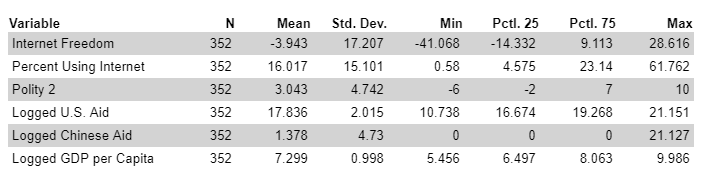
\includegraphics[scale=1.1]{628table2.png}
\end{figure}

A correlation matrix of the variables included in my regressions is given in Figure 2. As can be seen, there are a couple relatively strong relationships between variables. The variable for regime type, ``Polity 2,'' has a correlation of 0.62 with ``Internet Freedom'' while ``Logged GDP per Capita'' has correlation of 0.65 with the variable measuring internet development, ``Percent Using Internet.'' While possible, I do not think that these correlations are high enough to warrant concerns over multicollinearity or the lack of linear independency in the data. Interestingly, ``Logged U.S. Aid'' appears somewhat negatively correlated with ``Logged GDP per Capita'' and ``Percent Using Internet'' is somewhat positively correlated to ``Internet Freedom.''

\pagebreak
\subsubsection*{Figure 2}
\begin{figure}[htbp]
    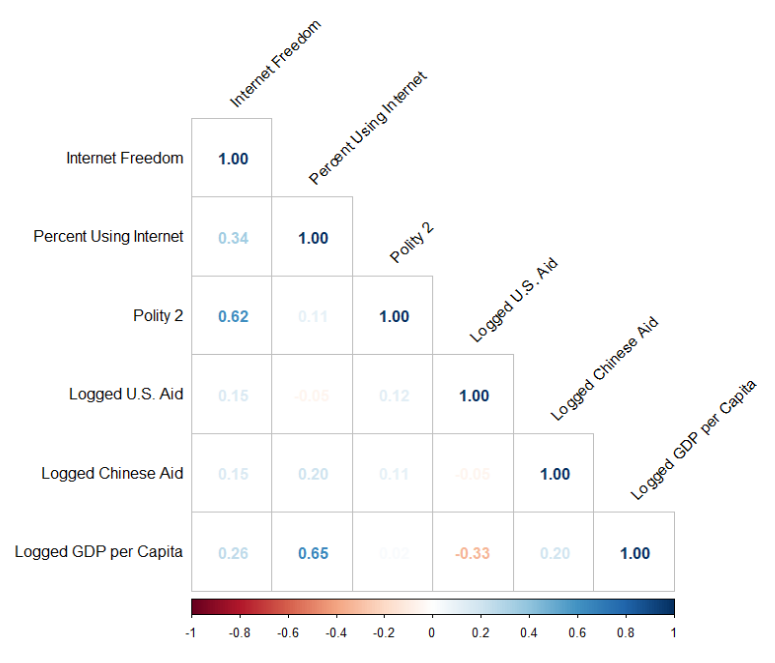
\includegraphics[scale=0.7]{628plot3.png}
\end{figure}

\subsection*{Estimation}
I chose to use ordinary least squares (OLS) for my estimator while employing two-way fixed effects at the country and year level. In choosing fixed effects, I used non-nested model comparison tests that suggested fixed effects to be superior to both no effects and random effects. After testing for heteroskedasticity, I included country-clustered standard errors.

\pagebreak
\section*{Results}
Table 2 displays regression results from a model with and without an interaction between internet freedom and logged Chinese foreign aid.

\subsection*{Table 2}
\begin{table}[!htbp] \centering 
  \caption*{Logged U.S. Aid and Covariates with Two-way Fixed Effects and Clustered SE's on Country} 
  \label{} 
\begin{tabular}{@{\extracolsep{5pt}}lcc} 
\\[-1.8ex]\hline 
\hline \\[-1.8ex] 
 & \multicolumn{2}{c}{Logged U.S. Aid} \\ 
\cline{2-3} 
 & Model 1 & Model 2 \\ 
\hline \\[-1.8ex] 
 Internet Freedom & 0.021$^{***}$ & 0.021$^{***}$ \\ 
  & (0.008) & (0.008) \\ 
  & & \\ 
 Logged Chinese Aid & 0.006$^{*}$ & 0.006$^{*}$ \\ 
  & (0.003) & (0.003) \\ 
  & & \\ 
 Logged GDP per Capita & 0.045 & 0.045 \\ 
  & (0.471) & (0.472) \\ 
  & & \\ 
 Percent Using Internet & $-$0.013 & $-$0.013 \\ 
  & (0.009) & (0.009) \\ 
  & & \\ 
 Polity 2 & 0.004 & 0.004 \\ 
  & (0.031) & (0.031) \\ 
  & & \\ 
 Internet Freedom $\cdot$ Logged Chinese Aid &  & 0.00000 \\ 
  &  & (0.0002) \\ 
  & & \\ 
\hline \\[-1.8ex] 
Observations & 352 & 352 \\ 
R$^{2}$ & 0.038 & 0.038 \\ 
Adjusted R$^{2}$ & $-$0.140 & $-$0.144 \\ 
F Statistic & 2.370$^{**}$ (df = 5; 296) & 1.968$^{*}$ (df = 6; 295) \\ 
\hline 
\hline \\[-1.8ex] 
\textit{Note:}  & \multicolumn{2}{r}{$^{*}$p$<$0.1; $^{**}$p$<$0.05; $^{***}$p$<$0.01} \\ 
\end{tabular} 
\end{table}

\pagebreak
Seems to support for $H_{1_b}$ and $H_{2a}$. In other words, seems that the U.S., in response to Chinese foreign aid, is using a intrastate competition strategy in competing with China and trying to increase IF in a trickle down manner.

\pagebreak
Figure 3 shows the marginal effect of internet freedom on logged U.S. foreign aid.

\subsection*{Figure 3}
\begin{figure}[htbp]
    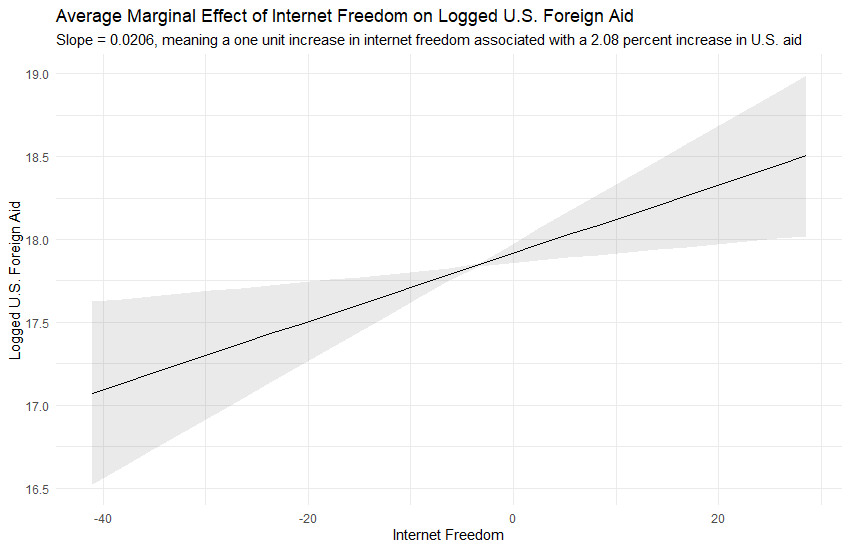
\includegraphics[scale=0.7]{628plot1.png}
\end{figure}

\pagebreak
Figure 4 graphs the marginal effect of logged Chinese foreign aid on logged U.S. foreign aid.

\subsection*{Figure 4}
\begin{figure}[htbp]
    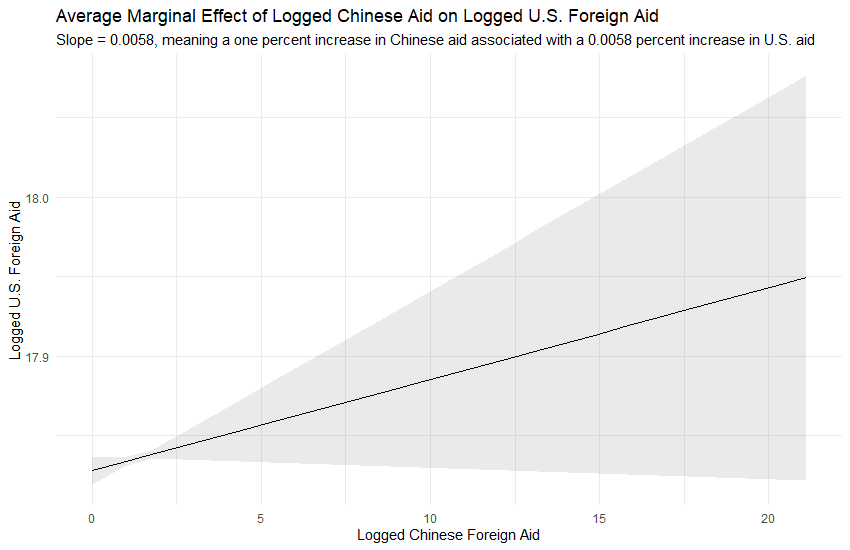
\includegraphics[scale=0.7]{628plot2.png}
\end{figure}
\pagebreak 

\section*{Discussion}
Talk about implications of trickle-down, intrastate strategy...

Why U.S. might be interested in IF.

Is U.S. response effective at keeping China out? Probably not, although they are ramping up efforts.

\section*{Conclusion}

\pagebreak
\section*{Appendix}
The entry game described in the theory section (Figure 1) is solved via backwards induction. If $China$ chooses to $Enter$, the $Donor$ chooses to $Spend$ if and only if (iff):

\begin{tabular}{c l}
    $\frac{\pi}{\gamma}-c > -1$ &  Condition for $Donor$ to $Spend$, from the payoffs on $Spend$ and $\neg Spend$, respectively.\\
    $\frac{\pi}{c-1} > \gamma $ & Isolating $\gamma$.\\
\end{tabular}

Where $\gamma \in (0,1]$. As $\gamma$ gets arbitrarily small, $\pi$ goes to infinity. 

\nocite{mechkova2022a}
\nocite{pemstein2022}
\nocite{coppedge2022}
\nocite{coppedge2022a}
\nocite{coppedge2022b}
\nocite{coppedge2022c}
\nocite{coppedge2022d}
\pagebreak
\printbibliography
\end{document}